\subsection{The Synthetic Population}
\label{subsec:synthetic_population}

We build a synthetic population based on the German microcensus \citep{FDSAeDBUDL2018}.
We only use private households, i.e. exclude living arrangements such as nursing homes as
non-private households vary widely in size and it is very difficult to know which
contacts take place in such living arrangements.

We sample households to build our synthetic population of over one million households
keeping for each of the 2.3 million individuals their age, gender, occupation and whether
they work on Saturdays and Sundays. For each household we draw its county and set the
corresponding federal state.% we draw the county because county is not part of the campus file

We randomly assign 35\% of children below three to attend a nursery \citep{Destatis2020}.
For children between three and six years old, we assume all go to preschool (officially
92.5\% according to \cite{Destatis2020}).
% nurseries and preschools
Children that attend a nursery meet in groups of four \citep{BertelsmannStiftung2019}
plus one adult care taker every weekday when there are no school vacations. Preschool
children meet in groups of nine \citep{BertelsmannStiftung2019} with two adult care
takers. These groups are mixed with respect to age but all belong to the same state and
mostly to the same county.

% school
Every child that goes to school is part of three different classes that meet every day on
weekdays when there are no vacations and no school policies are in place.\footnote{We
implement vacations on the federal state level.} Each class consists of approximately 23
students \citep{OECD2013} and two teachers. All students in a class are of the same age
and live in the same state and mostly also in the same county. In addition, each
child gets assigned a value that captures his or her need to attend nursery, preschool or
school. This allows us to capture various degrees of emergency care that can be granted
while educational facilities are closed or are on some kind of rotating schedule.

% workers
Workers are assigned to a daily meeting work group. The group sizes vary to match the
number of daily repeating work contacts reported by working individuals in
\cite{Mossong2008}. These groups only consist of workers that work in the same county.
For a distribution of the number of daily recurring work contacts see
Figure~\ref{fig:n_contacts_work_daily_recurrent}. To match the number of weekly work groups
we match each worker with up to 14 other workers into pairs to match the number of
reported weekly work contacts shown in Figure~\ref{fig:n_contacts_work_weekly_recurrent}.
Each pair is assigned a weekday on which they always meet in the absence of work
policies. 80\% of these contacts are individuals from the same county.
% work contact priority
In the same way children have an educational priority determining if they are entitled to
emergency care workers are assigned a work contact priority that captures how necessary
their work is and to which degree they can work from home. This means that it's always
the same individuals that continue to have work contacts when work from home mandates of
a certain strictness are in place.

% other recurring contacts
In addition to creating groups for educational facilities and work we also have other
recurring contacts to represent things like groups of friends or sports teams that
practice regularly together. Both daily and weekly groups are created analogously to the
work groups but matching the numbers in Figure~\ref{fig:n_contacts_other_daily_recurrent}
and Figure~\ref{fig:n_contacts_other_weekly_recurrent}. In addition, since leisure
contacts are highly assortative by age all individuals that have a daily leisure contact
are matched with a person not only from the same county but also from the same age group.

% individual responses
The individuals in our population can react to events such as developing symptoms that
are typical of CoViD-19, a positive PCR test or a positive rapid test by reducing their
contacts. To determine who would reduce their contacts in such a situation or demand a
rapid test we introduce a quarantine compliance parameter. Similarly, we introduce a
rapid test compliance parameter that determines in which order individuals start
demanding rapid tests when rapid tests become increasingly available. This makes sure
that when for example only 10\% of workers get tested, it's the same workers that have
access to tests every week.

% vaccination rank
Lastly, for the distribution of vaccinations every individual is assigned a vaccination
group and a vaccination rank from that group that creates a complete vaccination queue
over the population including a share that refuses to be vaccinated ($\xi$) which we
calibrate to  15\% \citep{RKI2021c}. The vaccination groups are created to match the
recommendations by the Ständige Impfkommission \citep{VygenBonnet2020}.\footnote{We cover
that teachers were prioritized more than recommended by the commission.} To cover that
the Pfizer-BioNTech vaccine was later approved for younger age groups we put adolescents
and children into two groups that follow after the general population. These groups do
not become eligible within our simulation frame until June. The way vaccinations are
rolled out in our model is shown in Figure~\ref{fig:vaccinations_by_age_group}.

\begin{figure}[ht]   % vaccinations by age group
  \centering
  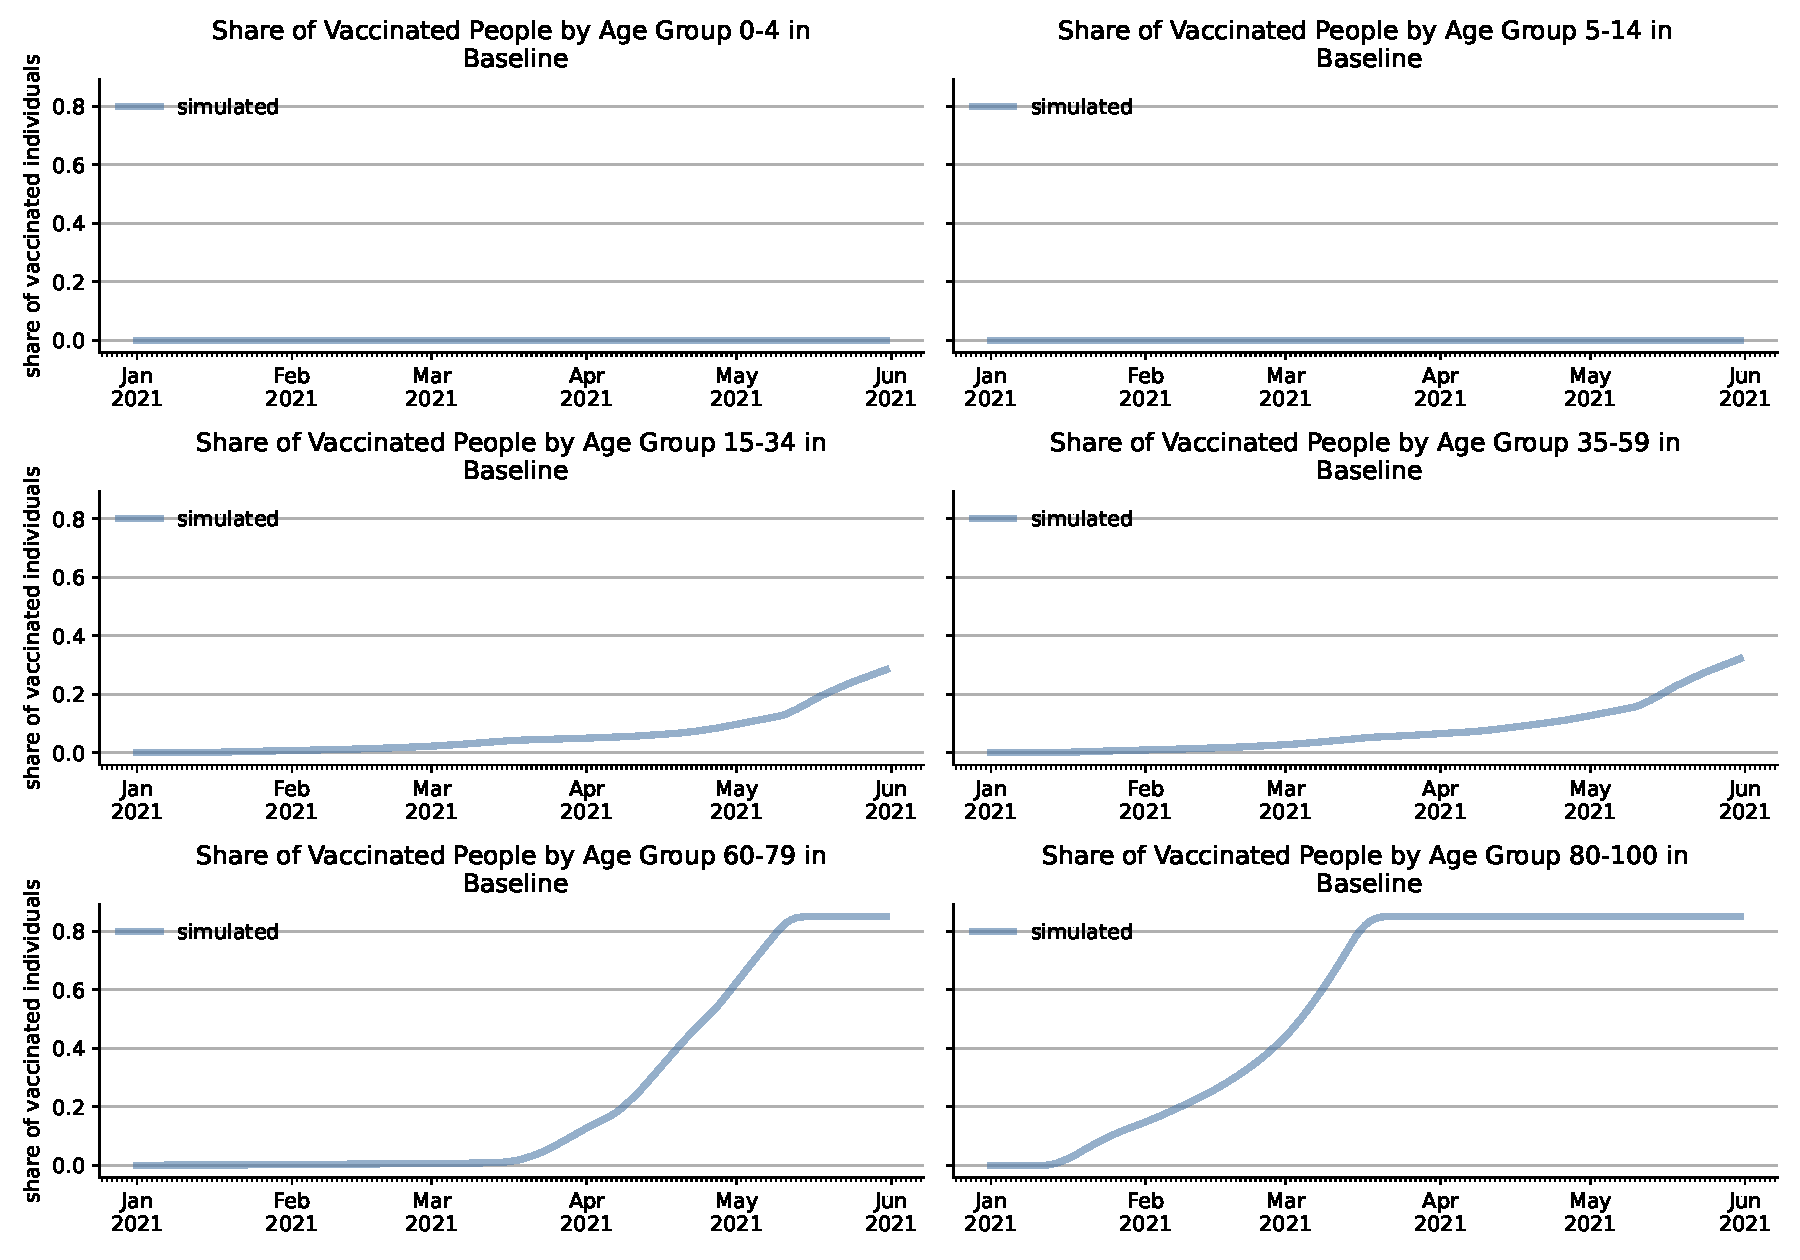
\includegraphics[width=\textwidth]{figures/results/figures/vaccinations/spring_baseline}
  \caption{Vaccination Rates by Age Group}
  \floatfoot{\noindent \textit{Note:} An individual's vaccination priority depends on her
  work contact priority, her age group and a random component to capture medical
  preconditions like diabetes. 15\% of the population refuse to be vaccinated ($\xi$).
  Adolescents would be vaccinated after the general population and children last. The
  figure clearly shows that the first vaccinations go to some workers with very high work
  contact priority and to the 80 to 100 age group followed by the 60 to 79 year olds.
  Both groups are saturated with vaccinations by mid March and start of May respectively.
  By June a third of the younger adults have received the vaccination but these groups
  still remain far from herd immunity thresholds.}
  \label{fig:vaccinations_by_age_group}
\end{figure}

\FloatBarrier
